%% content.tex
%%

%% ==============================
\chapter{This is a Chapter}
\label{ch:Intro}
%% ==============================

\section{This is a section}
This is some text referencing some \autoref{tab:severity}.

This only references the label number \ref{tab:severity}.



\subsection{This is a subsection}
\label{aLabel}
This is how citations can look: 
\begin{itemize}
\item \cite{Koeltzsch}\\
\item \parencite{Koeltzsch}\\
\item \textcite{Koeltzsch}\\
\end{itemize}









\begin{table}[h]
    \centering
    \caption{Severity of failure conditions~\cite[p. 779]{CS-25}}
    \begin{tabular}{c|ccccc}
        \toprule
         peeepee & poopoo \\
         example & 1 \\
    \end{tabular}
    \label{tab:severity}
\end{table}


\begin{figure}[h]
    \centering
    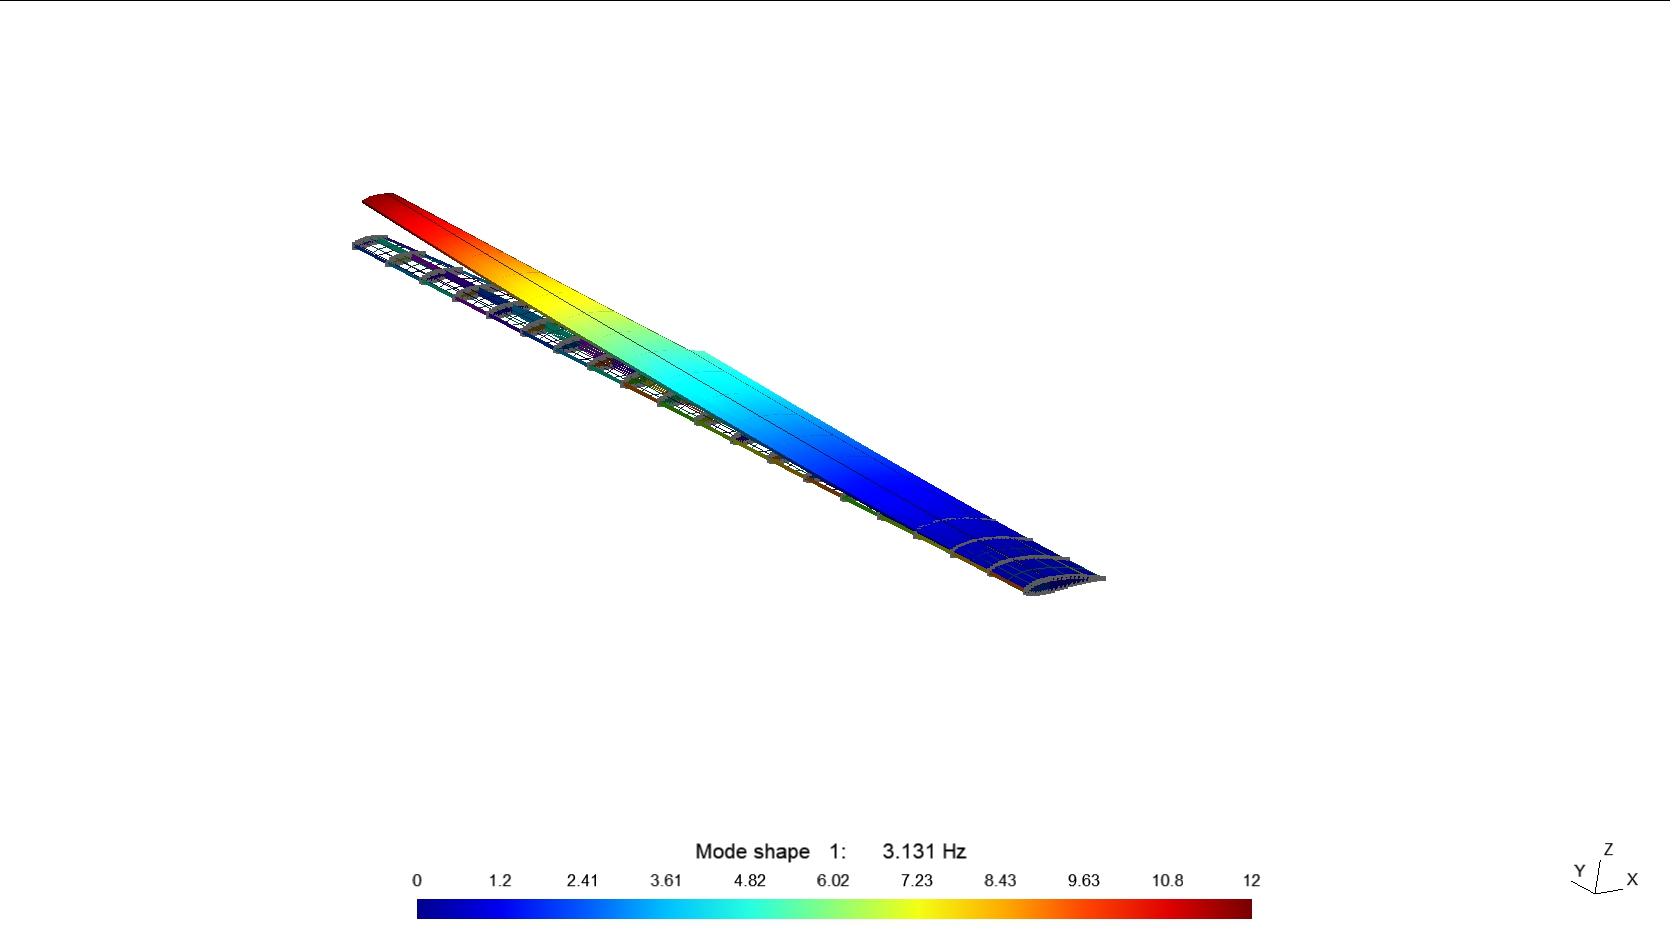
\includegraphics[width=.5\textwidth]{figures/mode1.jpg}
    \caption{The inverse relationship between probability and severity~\cite{CS-25}}
    \label{fig:inverseRelationship}
\end{figure}




